\documentclass{eceasst}
% This is an empty ECEASST article that can be used as a template
% by authors.
% Just uncomment the appropriate frontmatter commands and provide
% the parameters.

% Required packages
% =================
% Your \usepackage commands go here.
\usepackage{multirow}
\usepackage{listings}
\usepackage{amsmath}  % for equation*
\usepackage{array}    % for tabular
\usepackage{verbatim} % for comment
\usepackage{wrapfig}
\usepackage[final]{microtype}
\usepackage{tabularx}

\newcommand\forAll[1]{\forall \, #1 \, . \,}
\newcommand\forAllII[2]{\forall \, #1 \, #2 \, . \,}

\newcommand\propno[1]{(\emph{#1})}
\newcommand\hs[1]{\texttt{#1}}

\lstnewenvironment{code}[1][]
  {\noindent
   \vspace{-0.5\baselineskip}
   \lstset{basicstyle=\ttfamily,
           frame=single,
           language=Haskell,
           keywordstyle=\color{black},
           #1}
   \fontsize{8pt}{8pt}\selectfont}
  {}

% Volume frontmatter
% ==================
% Volume frontmatter for AVoCS 2015
% =====================================
\volume{72}{2015} % Volume number and year
\volumetitle{% Title of the volume (optional)
Proceedings of the\\
15th International Workshop on\\
Automated Verification of Critical Systems
(AVoCS 2015)}
\volumeshort{% Short title of the volume (optional)
Proc.\ AVoCS 2015}
\guesteds{% Multiple guest editors
Gudmund Grov, Andrew Ireland}


% Article frontmatter
% ===================
\title{Conditional Lemma Discovery and Recursion Induction in Hipster} % Title of the article
%\short{} % Short title of the article (optional)
%\author{\autref{1}\sponsor{}} % Authors and references to addresses
\author{Irene Lobo Valbuena and Moa Johansson}
%\institute{\autlabel{1}} % Institutes with labels
\institute{\email{lobo@student.chalmers.se},  \email{moa.johansson@chalmers.se} \\
Departement of Computer Science and Engineering \\Chalmers University of Technology, Gothenburg, Sweden.}

\abstract{Hipster is a theory exploration tool for the proof assistant Isabelle/HOL. It automatically discovers lemmas about given recursive functions and datatypes and proves them by induction. Previously, only equational properties could be discovered. Conditional lemmas, for example required when reasoning about sorting, has been beyond the scope of theory exploration. In this paper we describe an extension to Hipster to also support discovery and proof of conditional lemmas.

We also present a new automated tactic, which uses \emph{recursion induction}. Recursion induction follows the recursive structure of a function definition, as opposed to structural induction, which follows that of the datatype. We find that the addition recursion induction increases the number of proofs completed automatically, both for conditional and equational statements. } % Abstract of the article

\keywords{theory exploration, automated induction, interactive theorem proving} % Keywords for the article

\begin{document}
\maketitle

% Main part of your article
% =========================
\section{Introduction}
\label{sec:intro}

Theory exploration is a technique for automatically discovering new interesting lemmas in a formal mathematical theory development.
%
These lemmas are intended to help constructing a richer background theory about the concepts at hand (e.g. functions and datatypes) which can be useful both to enhance the power of automation as well as being of use in interactive proofs \cite{mathsaid,isacosy,isascheme}.
%
Theory exploration has proved particularly useful for automation of inductive proofs \cite{hipspecCADE}. This work builds on Hipster \cite{hipster}, an interactive theory exploration system for the proof assistant Isabelle/HOL \cite{isabelle}.
%
It can be used in two modes, either \emph{exploratory mode} to generate a set of basic lemmas about given datatypes and functions, or in \emph{proof mode}, where it assists the user by searching for missing lemmas needed to prove the current subgoal.
%
To generate conjectures, Hipster uses as a backend the HipSpec system, a theory explorer for Haskell programs \cite{hipspecCADE}.
%
Proofs are then performed by specialised tactics in Isabelle/HOL. Hipster has been shown capable of discovering and proving standard lemmas about recursive functions, thus speeding up theory development in Isabelle.
%
However, lemma discovery by theory exploration has previously been restricted to equational properties.
%
In this paper we take the first steps towards lifting this restriction and exploring also conditional conjectures.
%
Conditional lemmas are necessary if we for example want to prove properties about sorting algorithms.
%
As an example, consider the proof of correctness for insertion sort:
%
%\begin{small}
\begin{center}
\isaCode{theorem isortSorts: "sorted (isort xs)"}
\end{center}
%\end{small}
%
To prove this theorem by induction will in the step-case require a lemma telling us that if a list is sorted, it remains so after an additional element is inserted:
%
\begin{center}		
\isaCode{lemma "sorted xs $\Longrightarrow$ sorted (insert x xs)"}
\end{center}
%
Discovering this kind of conditional lemmas introduces a big challenge for theory exploration.
%
First of all, the search space greatly increases: what statements should be picked as potentially interesting side-conditions to explore?
%
Secondly, as our theory exploration system relies on generation of random test-cases, we also need to ensure that we perform tests where the condition evaluates to true, otherwise we may miss conditional equations as the theory exploration system might place the relevant terms in different equivalence classes (see Example 2 on p. \pageref{example2}).

As Hipster is designed as an interactive system, we avoid the first problem by asking the user to specify under which condition theory exploration should occur.
%
In the example above, this would require the user to tell Hipster that the predicate \isaCode{sorted} is an interesting pre-condition, in addition to which function symbols should be explored in the bodies of lemmas.
%
The rest of the process is however automatic.
%
We describe it in more detail in \S \ref{sec:conditionals} 

The second contribution of this paper is a new automated tactic for \emph{recursion induction} (see e.g. \S3.5.4 of \cite{isabelle}).
%
Previously, Hipster only supported structural induction over the datatypes, but has now been extended with a new tactic that uses recursion induction, following the termination order of function definitions instead of the datatype.
%
This has shown to be useful for many proofs that previously failed, but can also provide shorter proofs in some cases.
%
The new recursion induction tactic is described in \S \ref{sec:rec-ind}.
%
It is used by Hipster during automated theory exploration, but can equally well be applied as a powerful regular tactic by a human user working in Isabelle.


%Background, explaining how Hipster works
\section{Hipster}
\label{sec:background}
This section provides a description of how Hipster works and how its subsystem QuickSpec generates conjectures.

\subsection{Theory Exploration in Hipster}
Figure \ref{fig:hipster} gives an overview of the Hipster system.
%
Starting from an Isabelle theory file that defines a set of datatypes and functions, the user calls Hipster on a list of functions about which she is interested in finding lemmas.
%
The workings of Hipster can be divided up into three stages:
\begin{enumerate}
\item Generation of Haskell code. 
\item Theory exploration in Haskell.
\item Proof in Isabelle.
\end{enumerate}

\begin{figure}[htbp]
\begin{center}
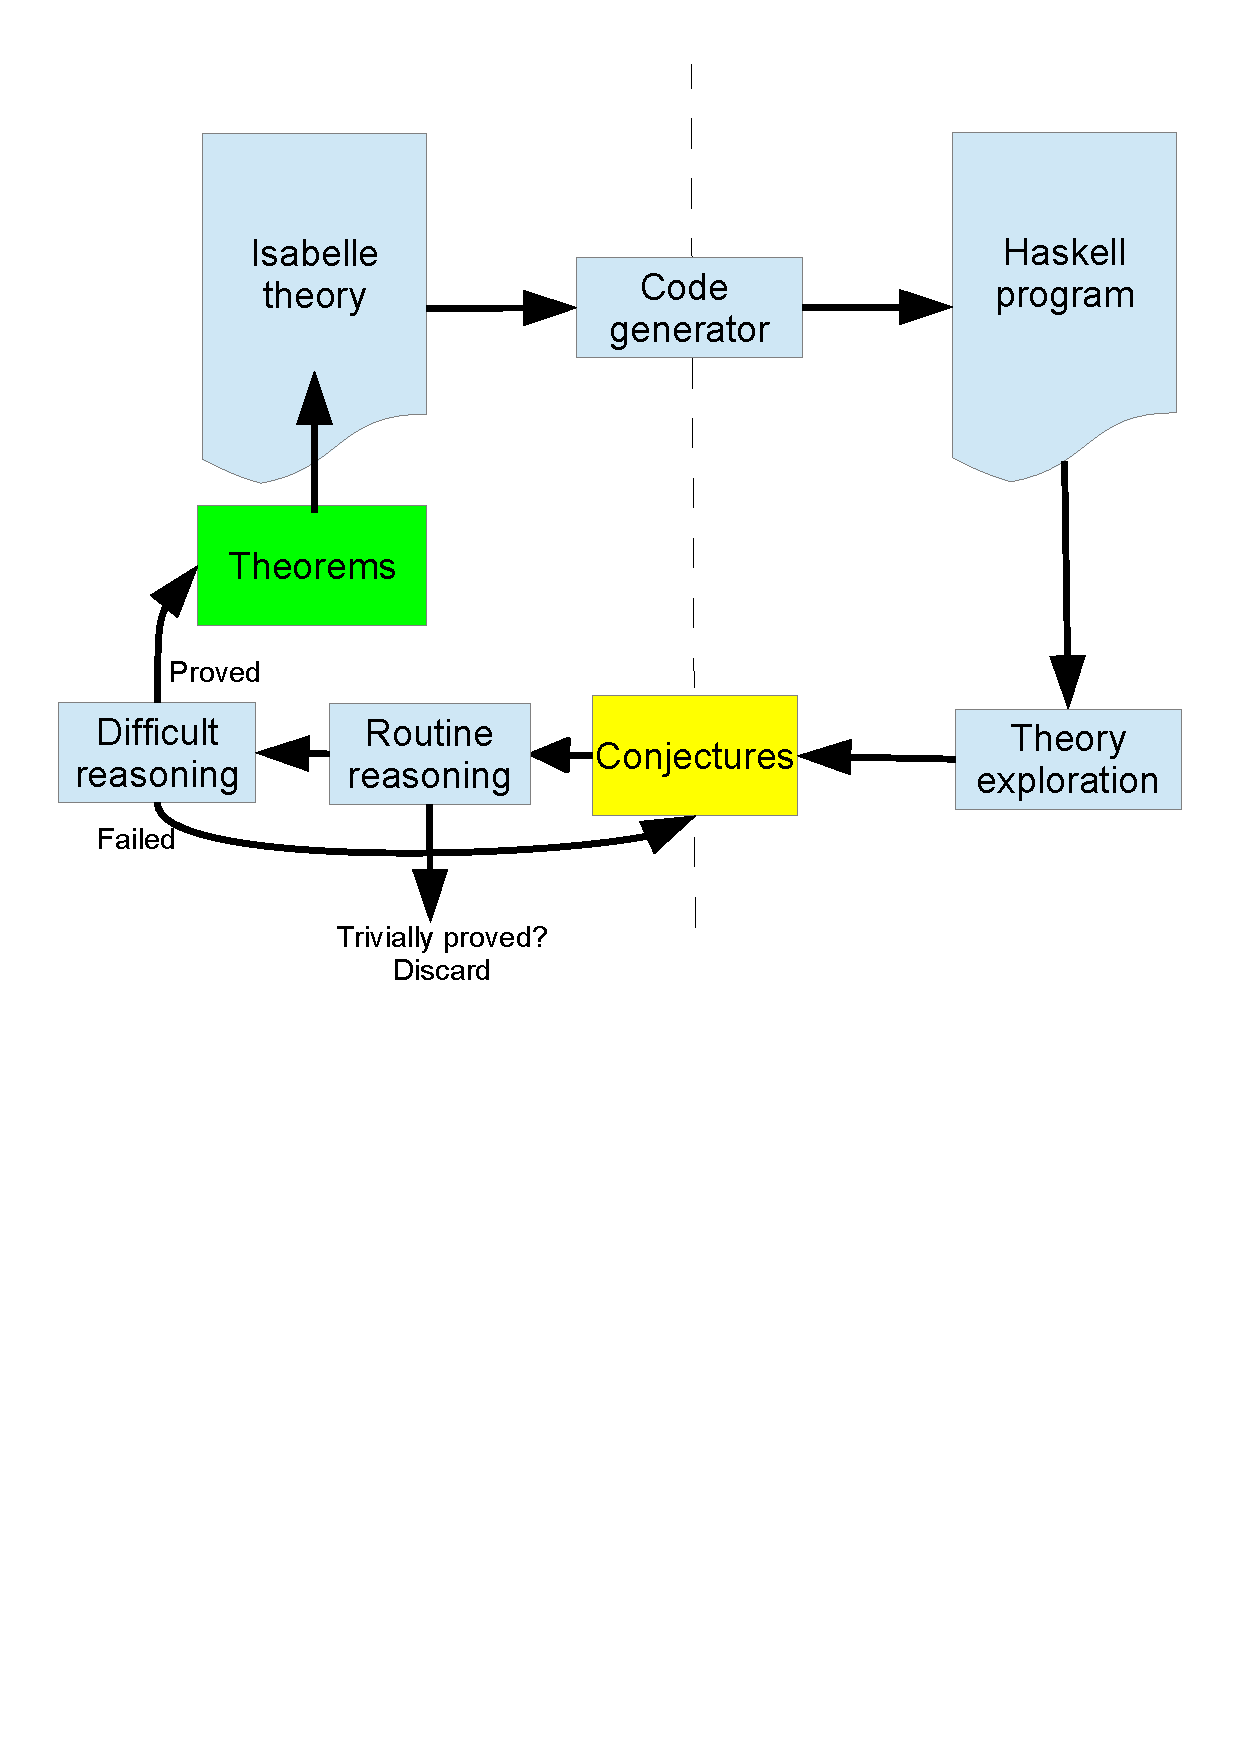
\includegraphics[scale=0.4]{hipster}
\caption{Overview of Hipster}
\label{fig:hipster}
\end{center}
\end{figure}

Hipster uses Isabelle's code generator \cite{codegen2}, to translate the theory to a Haskell program.
%
Hipster then employs the theory exploration system HipSpec as a backend for generating conjectures.
%
While HipSpec can be used also as a fully fledged theorem prover, Hipster only uses its conjecture generation subsystem QuickSpec \cite{quickspec}, and performs proofs inside Isabelle.
%
Isabelle is an LCF-style prover, which means that it is based on a small core of trusted axioms, upon which subsequent proofs must be built.
%
Therefore, any proofs found outside Isabelle, e.g. by HipSpec, would have to be reconstructed inside Isabelle anyway.
%
Hence it is easier for Hipster to simply use Isabelle for proofs in the first place. 

Not all conjectures returned from QuickSpec are interesting.
%
Hipster is parametrised by two tactics, which can be set by the user: one for \emph{routine reasoning} and one for \emph{difficult reasoning}.
%
Conjectures solved by routine reasoning are deemed trivial and discarded, while those requiring more difficult reasoning are displayed to the user and included in the Isabelle theory so they can be used in subsequent proofs if necessary.
%
In the context of this paper, routine reasoning is first-order equational reasoning and simplification, while difficult reasoning involves some kind of induction. If a conjectur is not immediately provable, Hipster will place it at the end of the list of open conjectures and will try it again if it has found some additional lemmas.
%
Occasionally, Hipster might discover some conjecture which it does not manage to prove automatically, because not even its tactic difficult reasoning is strong enough. Such an open conjecture would also be displayed to the user, who can then choose to perform an interactive proof in Isabelle, perhaps employing other tactics or lemmas than those currently available to Hipster.


\subsection{Conjecture Generation in QuickSpec}
% XXX: "by default three per type" ?
QuickSpec takes as input a set of functions and variables (by default three per type), and generates all type-correct terms up to a given limit (by default depth three).
%
The number of variables and term-depth limit can be adjusted by the user.
%
QuickSpec then proceeds to divide the generated terms into equivalence classes, so that each equivalence class eventually represents a set of equations.
%
Initially, all terms of the same type are in the same equivalence class. QuickSpec then uses QuickCheck \cite{quickcheck}, to generate random ground values for the variables in the terms, and evaluates the result.
%
If two terms in an equivalence class turn out to evaluate differently, the equivalence class is split accordingly.
%
The process is then repeated until the equivalence classes stabilise (after several hundred different random tests), which means that we usually have quite a high confidence in that the conjectures produced are probably true, even though they are not yet proved.  

% This paragraph could possibly be in the next section on conditional lemmas, but it feels like it belongs to the Background section in a way...
%The support in QuickSpec for generating conditional conjectures (implications) is still rather basic.
%%
%In this case, QuickSpec will in addition to the other input require the user to specify a predicate to use as the premise of an implication.
%%
%Term generation proceeds as described above, but testing takes the given predicate into account.
%%
%Here, we are only interested in tests with values that make the premise true, otherwise we may split the equivalence classes when they should not be split.
%%
%QuickCheck uses special functions called \emph{generators} to produce random values of a given type.
%%
%If using QuickSpec directly in Haskell, the user can program special purpose generators that could be made to only produce values satisfying a given predicate.
%%
%In Hipster, however, these generator functions are simpler as they have to be automatically derived together with the Haskell code.
%%
%Tests not satisfying the premise are simply discarded during conditional exploration, which means that we typically must generate more tests than for equational conjectures.
%%
%Also, the risk of some non-theorem slipping through is slightly higher, but as Hipster then attempts to prove all conjectures, such a statement would be caught in the proving phase.
%%
%Automatically generating customised generator functions is further work. 

%%% Example if there is space %%%
\paragraph*{Example 1.}
\label{example1}
As a small example, consider a theory exploration attempt where we have asked Hipster for lemmas about a function \isaCode{isort} implementing insertion sort.
%
%We are furthermore interested in the case with the condition that the predicate \isaCode{sorted} holds (for one variable). %Among the terms generated by QuickSpec are for example: \isaCode{xs}, \isaCode{sort xs}, \isaCode{sort(sort xs)}. 
%QuickSpec first performs one pass looking for plain equations, then a second where it considers the condition \isaCode{sorted xs}. 
%
%We start with the first phase, where QuickSpec investigates non-conditional conjectures.
%%
Among the terms generated by QuickSpec are those in the table below.
%
Initially, all terms are placed in the same equivalence class.
%
Suppose QuickSpec generates the random value \isaCode{xs} $\rightarrow$ \isaCode{[3,1]}.     

\vspace{2 mm}

\noindent \begin{tabularx}{\textwidth}{l  X  X  X}
 & Term & Ground Instance & Value \\
 \hline
1 \quad &\isaCode{isort xs} & \isaCode{isort [3,1]} & \isaCode{[1,3]} \\
2 \quad&\isaCode{isort (isort xs)} &\isaCode{isort (isort [3,1])} & \isaCode{[1,3]}\\  
3 \quad &\isaCode{xs} &\isaCode{[3,1]} & \isaCode{[3,1]} \\
\end{tabularx}

\vspace{2 mm}

\noindent As not all terms evaluate to the same value, they should no longer be in the same equivalence class. We thus split the terms into two new equivalence classes: terms 1 and 2 evaluate to the same value and remain together, while term 3 is separate.
%
After this, no subsequent tests further split these equivalence classes, and we can read off the equation: \isaCode{isort(isort xs) = isort xs}.  
%
%In the second phase, QuickSpec performs a new exploration, this time requiring the predicate \isaCode{sorted xs} to hold for all test values.
%%
%Suppose we test with the sorted list: \isaCode{xs $\rightarrow$ [1,2]} (other non-sorted values for \isaCode{xs} would be discarded).       
%
%\vspace{2 mm}
%
%\noindent \begin{tabularx}{\textwidth}{l  X  X  X}
% & Term & Ground Instance & Value \\
% \hline
%1 \quad &\isaCode{sort xs} & \isaCode{sort([1,2])} & \isaCode{[1,2]} \\
%2 \quad &\isaCode{sort (sort xs)} &\isaCode{sort (sort [1,2])} & \isaCode{[1,2]}\\
%3 \quad &\isaCode{xs} &\isaCode{[1,2]} & \isaCode{[1,2]} \\
%\end{tabularx}
%
%\vspace{2 mm}
%
%\noindent This time, all terms evaluate to the same value on all tests where the list is sorted, so all three terms remain in the same equivalence class.
%%
%QuickSpec realises that there is no point producing the conjecture \isaCode{sorted xs $\Longrightarrow$ sort (sort xs) = xs}, as this is subsumed by the non-conditional equation discovered in the first phase.
%%
%It will however produce the additional conjecture \isaCode{sorted xs $\Longrightarrow$ sort xs = xs}, which clearly only holds if the list is already sorted.
%



% Conditional lemmas, with a worked example
\section{Conditional Lemmas}

% Recursion induction
\section{Automating Recursion Induction}

% The experimental results
\section{Evaluation}

\section{Related Work}

\section{Conclusion and Further Work}


% Acknowledgements for colleagues, referees, ...
% ==============================================
%\begin{acknowledge}
%\end{acknowledge}

% Bibliography with BibTeX
% ========================
\bibliographystyle{eceasst}
\bibliography{bibfile}

\end{document}
